% 第4章
\section{システム設計(\textcolor{orange}{5\%})}
  \label{sec:system_design}
    \par
  
  \subsection{システム要件の定義(0\%)}
    \label{sec:definition_of_system_requirements}
      \par
  
      \subsubsection{ユーザー要件(0\%)}
        \label{sec:user_requirements}
          \par
          
      \subsubsection{機能要件(0\%)}
        \label{sec:functional_requirements}
          \par
          
      \subsubsection{非機能要件(0\%)}
        \label{sec:non-functionla_requirements}
          \par
      
  \subsection{全体アーキテクチャの設計(0\%)}
    \label{sec:overall_architecture_design}
      \par
      
      \subsubsection{システム構成図(0\%)}
        \label{sec:system_configuration_diagram}
          \par
          
      \subsubsection{データフローの設計(0\%)}
        \label{sec:data_flow_design}
          \par  
  
  \subsection{スマートロックの構築(0\%)}
    \label{sec:smart_lock_construction}
      \par 
      
      \subsubsection{ハードウェア設計(0\%)}
        \label{sec:hardware_design}
          \par
          
      \subsubsection{組み込みソフトウェアの開発(0\%)}
        \label{sec:embedded_software_development}
          \par
          
      \subsubsection{通信プロトコルの選定(0\%)}
        \label{sec:selection_of_communication_protocols}
          \par
          
  \subsection{マッチングモデルの設計(0\%)}
    \label{sec:matching_model_design}
      \par

      \subsubsection{数理最適化モデルの定式化(\textcolor{green}{100\%})}
        \label{sec:数理最適化モデルの定式化}
          \par $\Box$ 変数や制約の数、計算複雑性について触れる。
          \par シェアサイクルサービスをCtoC化することによる特徴として,サービスを提供するために大量の自転車を予め確保する必要性がなく,個人が所有している未使用の自転車を有効活用することができる点や,都市部と地方で設置数に偏りが生じやすいポートに依存せず,ポートがない場所でも乗り捨てが可能となり,移動自由度の向上が期待できる点が挙げられる.また,自転車保有者側の観点においても,自転車を利用していない期間にそれをユーザに貸し出すことで,自身のリソースを有効活用できると捉えることもできる.一方で,ユーザに対して適切な自転車が割り当てられない場合や,既存のシェアサイクルシステムのようにユーザが好みの自転車を自由に選択することができる状況下においては,乗り捨てられた自転車とその保有者との位置関係が未知数となり,自転車を再配置する際に多くのコストを要することが想定される.
          
          \par そこで,個人所有の自転車を効率的にシェアし,乗り捨て可能なシェアサイクルシステムを実現するため,数理最適化ベースの自転車割り当てモデルを設計し,構築する.ユーザに自転車を割り当てるアルゴリズムを数式としてモデル化し,それに基づいて自転車割り当て処理が実行されるため,乗り捨て可能な個人所有自転車のシェアリングにおいて的確な割り当て結果を得ることが期待される.
          
          \par モデルの構築においては,整数計画法によるアルゴリズムを軸とする.
          
          \par 整数計画法は,一部または全ての決定変数が整数値のみをとるように制約された線形計画法である\scalebox{0.7}{\cite{wolsey2020integer}}.一方で,線形計画法では,変数は整数値以外も取ることができる.そのため,本研究でアプローチしているような整数計画問題を線形計画法を用いたプロセスで処理しようとすると,線形計画法による解が整数ではない場合,丸めた解が実行不可能または最適ではない可能性がある\scalebox{0.7}{\cite{hooker2024integer}}.整数計画法では,決定変数が整数であるべき多くの現実世界の状況をモデル化するのに役立つ\scalebox{0.7}{\cite{gomory1960integer}}.これらの観点を踏まえ,個人所有の自転車をユーザに割り当てる問題では,決定変数が「割り当てるか否か」のバイナリ変数であるべき問題であることより,整数計画法を用いたアルゴリズムを構築する.
          
          \par 前提条件として,本モデルが数理最適化ベースであることの利点を最大限活用するため,ユーザから自転車割り当てシステムに対するリクエストは1分間ストックし,ストックされたリクエストデータに対して毎分バッチ処理を実行する.また,シェアリングの対象は個人所有の自転車とし,ユーザ体験の観点において,移動自由度を向上させることを目的としてドックレスで乗り捨て可能なシステムを想定する.なお,乗り捨てによる自転車の不法駐輪等の法的な課題に関してはここでは考慮せず,あくまで自転車の割り当て問題として切り分けてモデリングする.
          
          \par 定式化で用いる集合やパラメータ,決定変数のそれぞれの記号と概説を表\ref{tab:記号の概説}に示す.ユーザリクエストの集合を$R$,シェアリングされる自転車の集合を$B$とする.ユーザ$r (r \in R)$に自転車$b (b \in B)$が割り当てられる前の初期状態として,ユーザとユーザがリクエストした時点での自転車の距離関係を表すパラメータを距離行列$d^{\text{init}}_{b,r}$とする.ユーザ$r (r \in R)$に自転車$b (b \in B)$が割り当てられ,ユーザが割り当てられた自転車に乗って移動したと仮定した場合のその後の自転車の位置と自転車の所有者までの距離関係を表すパラメータを距離行列$d_{b,r}$とする.
          
          \begin{table}[htbp]
            \caption{記号の概説}
            \label{tab:記号の概説}
            \centering
            \begin{tabular}{c p{6cm}}
              \hline 
              記号 & 説明 \\
              \hline
              $R$ & ユーザリクエストの集合 \\
              $B$ & シェアリングされる自転車の集合 \\
              $d^{\text{init}}_{b,r}$ & ユーザ $r(r \in R)$ と自転車 $b(b \in B)$ の割り当て前の距離行列\\
              $d_{b,r}$ & ユーザ $r (r \in R)$ に自転車 $b (b \in B)$ が割り当てられて移動した後の距離行列 \\
              $x_{b,r}$ & ユーザ $r (r \in R)$ に自転車 $b (b \in B)$ が割り当てられたか否かの二値変数行列 \\
              \hline
            \end{tabular}
          \end{table}
          
          \par 決定変数については,ユーザ$r (r \in R)$に自転車$b (b \in B)$が割り当てられたか否かの二値変数行列$x_{b,r}$とする.ユーザ$r$が自転車$b$を利用する場合に1,そうでなければ0のバイナリ値を持つ.
          
          \par 目的関数は\ref{equ:目的関数}式の通りに定義する.
          
          \begin{equation}\label{equ:目的関数}
            \min \left( \sum_{b \in B}\sum_{r \in R}d_{b,r}x_{b,r} - \alpha\sum_{b \in B}\sum_{r \in R}x_{b,r} \right)
          \end{equation}
          
          \begin{equation}\label{equ:移動後の距離最小化}
            \min \left( \sum_{b \in B}\sum_{r \in R}d_{b,r}x_{b,r} \right)
          \end{equation}
          
          \begin{equation}\label{equ:割り当て成功率最大化}
            \max \left(\sum_{b \in B}\sum_{r \in R}x_{b,r} \right)
          \end{equation}
          
          \par 第1項の部分については,\ref{equ:移動後の距離最小化}式に示す通り,ユーザが割り当てられた自転車に乗って移動した後の自転車とその自転車の所有者までの距離を最小化する.例えば,あるユーザからのリクエストがあった場合,そのユーザの現在地と目的地,リクエストされた時点での自転車とその自転車の所有者までの位置関係が図\ref{fig:ユーザと自転車の初期位置とリクエスト方向}の状態であったとする.なお,自転車の位置は自転車のアイコンで,自転車の所有者の位置は家のアイコンで表し,所有関係は色に対応している.この場合,\ref{equ:移動後の距離最小化}式に従うと,ユーザには緑色の自転車が割り当てられる.ユーザが移動した直後の状態が図\ref{fig:自転車割り当て・移動後の位置関係}に示す通りとなり,橙色の自転車が割り当てられた場合と比較して,点線で示した自転車とその自転車の所有者との距離の総和が小さくなる.
          
          \begin{figure}[htbp]
            \centering
            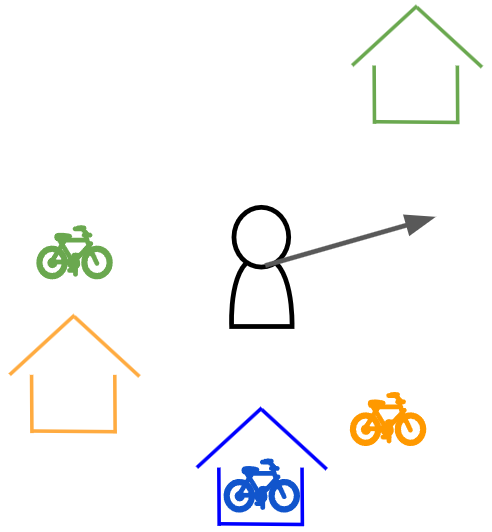
\includegraphics[scale=0.6]
            {figures/subjectFunction1-0.png}
            \caption{ユーザと自転車の初期位置とリクエスト方向}
            \label{fig:ユーザと自転車の初期位置とリクエスト方向}
          \end{figure}
          \begin{figure}[htbp]
            \centering
            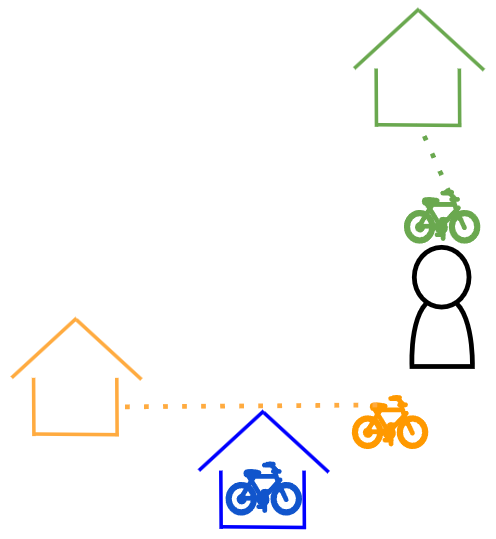
\includegraphics[scale=0.6]
            {figures/subjectFunction1-1.png}
            \caption{自転車割り当て・移動後の位置関係}
            \label{fig:自転車割り当て・移動後の位置関係}
          \end{figure}
          
          \par 第2項の部分については,\ref{equ:割り当て成功率最大化}式に示す通り,可能な限り多くのユーザに自転車を割り当てる最大化を行う.\ref{equ:移動後の距離最小化}式のみを目的関数として定義した場合,全ての自転車が所有者の手元にあるような極端な状況ではユーザに自転車を一切割り当てない選択をすることが,割り当て移動後の自転車とその自転車の所有者までの距離が最小化される結果となり,最適と判断されてしまう.サービスとしてもユーザに自転車が割り当てられることで初めて機能するため,\ref{equ:割り当て成功率最大化}式を目的関数の一部としている.
          
          \par なお,\ref{equ:移動後の距離最小化}式と\ref{equ:割り当て成功率最大化}式は最小化と最大化のトレードオフの関係にあるため,\ref{equ:割り当て成功率最大化}式に対してトレードオフの調整を行う重み$\alpha$を掛け合わせ,このトレードオフの最適値を探る.ただし,$\alpha$は非負であることを保証し,指定が無い場合は$\alpha=1$とする.\ref{equ:割り当て成功率最大化}式に対して$-\alpha$を掛け合わせることで,目的関数全体として最小化を行う.
          
          \par 制約条件は\ref{equ:半径制約}式から\ref{equ:人対自転車}式の通りに定義する.
          
          \begin{equation}\label{equ:半径制約}
            x_{b, r} \leq \mathbb{I}(d^{\text{init}}_{b, r} \leq 250), \forall b \in B, \, \forall r \in R
          \end{equation}
          
          \begin{equation}\label{equ:自転車対人}
            \sum_{r \in R}x_{b,r} \leq 1, \forall b \in B
          \end{equation}
          
          \begin{equation}\label{equ:人対自転車}
            \sum_{b \in B}x_{b,r} \leq 1, \forall r \in R
          \end{equation}
          
          \par \ref{equ:半径制約}式は,ユーザから半径250m以内の自転車のみを割り当てる制約を意味する.図\ref{equ:半径制約}に示すように,ユーザから半径250mの範囲外に位置する自転車は割り当ての対象外となる.\ref{equ:自転車対人}式は,図\ref{fig:自転車に割り当てられるユーザは1人以下}に示すように,自転車に割り当てられるユーザは1人以下であることを定義し,\ref{equ:人対自転車}式は,図\ref{fig:ユーザに割り当てられる自転車は1台以下}に示すように,ユーザに割り当てられる自転車は1台以下であることを定義する.これらの制約条件を設けることによって,ユーザから遠く離れた場所に位置する自転車の割り当てや,利用する自転車がユーザ同士で重複して割り当てられること,ユーザが複数台の自転車を利用して移動することを防ぐ.
          
          \begin{figure}[htbp]
            \centering
            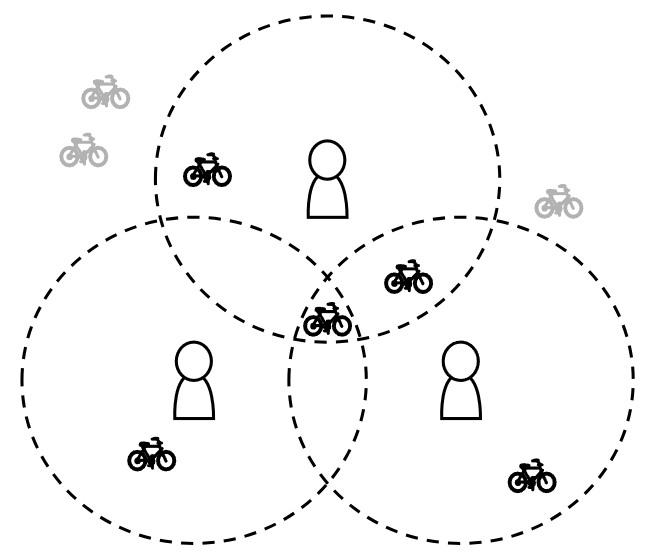
\includegraphics[scale=0.45]
            {figures/objectFunction1.png}
            \caption{割り当て許容距離に含まれている自転車の状態}
            \label{fig:割り当て許容距離に含まれている自転車の状態}
          \end{figure}
          
          \begin{figure}[htbp]
            \centering
            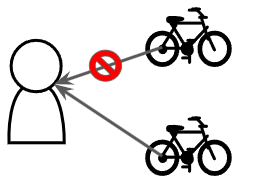
\includegraphics[scale=1.2]
            {figures/objectFunction2.png}
            \caption{自転車に割り当てられるユーザは1人以下}
            \label{fig:自転車に割り当てられるユーザは1人以下}
          \end{figure}
          
          \begin{figure}[htbp]
            \centering
            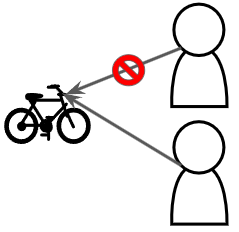
\includegraphics[scale=1.2]
            {figures/objectFunction3.png}
            \caption{ユーザに割り当てられる自転車は1台以下}
            \label{fig:ユーザに割り当てられる自転車は1台以下}
          \end{figure}

      \subsubsection{機械学習モデルの設計(0\%)}
        \label{sec:machine_learning_model_design}
          \par

  \subsection{APIの設計方針(0\%)}
    \label{sec:api_design_policy}
      \par

      \subsubsection{API機能の定義(0\%)}
        \label{sec:definition_of_api_function}
          \par

      \subsubsection{セキュリティと認証の設計(0\%)}
        \label{sec:security_and_authentication_design}
          \par
